\documentclass[10pt,a4paper]{article}
\usepackage[utf8]{inputenc}
\usepackage[italian]{babel}
\usepackage{amsmath}
\usepackage{amsfonts}
\usepackage{amssymb}
\usepackage{graphicx}
\usepackage{siunitx}
\usepackage[left=2cm,right=2cm,top=2cm,bottom=2cm]{geometry}
\newcommand{\rem}[1]{[\emph{#1}]}
\newcommand{\exn}{\phantom{xxx}}

\author{Gruppo 1.BN \\ Massimo Bilancioni, Alessandro Foligno, Giuseppe Zanichelli }
\title{Amplificatore a transistor}


\begin{document}

\date{4 ottobre 2018}
\maketitle

\section{Risposta a segnali sinusoidali di frequenza fissa}

Abbiamo scelto una frequenza di lavoro intorno ai $7.40$ \si{\kilo\hertz}.

a) 
\vspace{0.5cm}

i)  Abbiamo verificato l'inversione di fase per VOUT, la figura sotto riporta quanto osservato.

\begin{figure}[h]
	\centering
	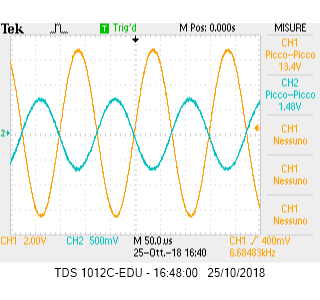
\includegraphics[scale=0.5]{oscilloscopio.png}

	
	
\end{figure}

ii)  Facendo una media dei guadagni per piccole  ampiezze diverse di VIN, otteniamo :\[A_v= (9.76\pm0.01) \]
  (VIN e VOUT sono stati misurati sui due canali differenti dell'oscilloscopio,per questo abbiamo considerato gli errori scorrelati)
\begin{table}[h]
	\centering
	\begin{tabular}{|c|c|c|}
		\hline 
		 VIN (\si{\volt}) &  VOUT (\si{\volt})   & VOUT/VIN\\
		\hline 
	$0.228 \pm  0.06 $& $2.20\pm 0.06$& $9.65 \pm 0.04$\\
	$0.320\pm 0.08 $& $3.12 \pm 0.08$& $9.75 \pm0.04$\\
	$0.528\pm 0.015 $& $5.14 \pm 0.15$& $9.73\pm 0.04$ \\
	$0.752\pm 0.021$& $7.32\pm 0.21$ & $9.73\pm 0.04$\\
	$1.02\pm 0.03 $& $10.2\pm 0.3$& $10\pm 0.04 $\\
	$1.27\pm 0.04$ & $12.3\pm 0.4 $& $9.69\pm 0.04 $\\

		\hline 
	\end{tabular} 
\end{table}

\begin{figure}[h]
	\centering
	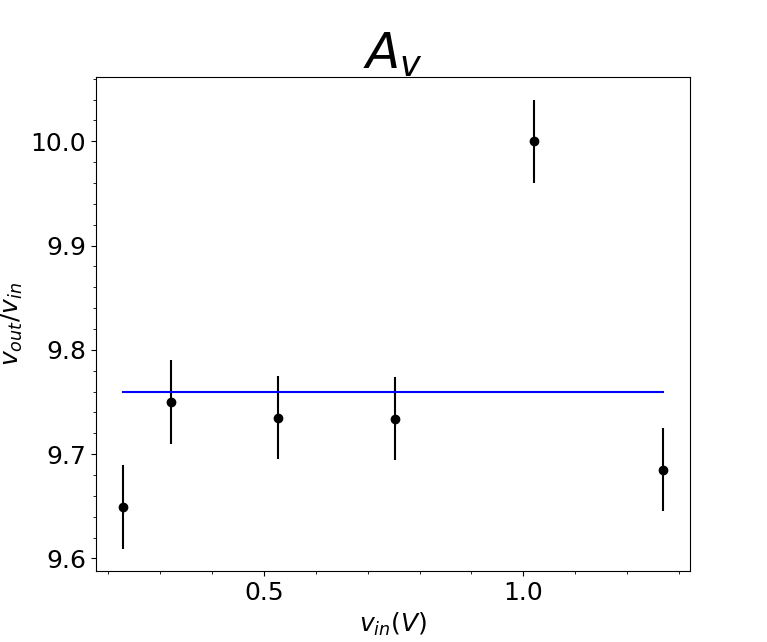
\includegraphics[scale=0.5]{guadagno.png}

	
	
\end{figure}

iii) Per un segnale in ingresso di circa $1.60$ \si{\volt}pp si iniziano a vedere distorsioni per VOUT.

iv)\begin{figure}[h]
	\centering
	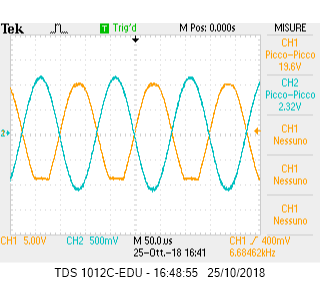
\includegraphics[scale=0.5]{clipping.png}

	
	
\end{figure}

	

\section*{Dichiarazione}
I firmatari di questa relazione dichiarano che il contenuto della relazione \`e originale, con misure effettuate dai membri del gruppo, e che tutti i firmatari hanno contribuito alla elaborazione della relazione stessa.

\end{document}